\documentclass[mathNotesPreamble]{subfiles}
\begin{document}
%\relscale{1.4} %TODO
\section{16.6: Integrals for Mass Calculations}
  Suppose we have two masses $m_1$ and $m_2$ on a beam (with no mass) that are distances $d_1$ and $d_2$ away from a pivot point. This beam will be balanced when $m_1d_1=m_2d_2$.
  \vspace*{10pt}
  \begin{center}
    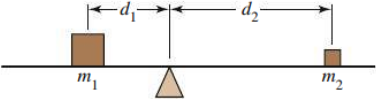
\includegraphics[width=0.45\linewidth]{images/briggs_16_06/fig16_64}
  \end{center}
  \vspace*{10pt}
  This concept can be used to to find the balance point $\bar{x}$ between 2 objects with masses $m_1$ and $m_2$:
  \begin{center}
    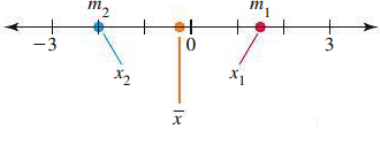
\includegraphics[width=0.45\linewidth]{images/briggs_16_06/fig16_65}
  \end{center}
  \[m_1\parens{x_1-\bar{x}}=m_2\parens{\bar{x}-x_2}\hspace*{5pt} \Rightarrow \hspace*{5pt} m_1\parens{x_1-\bar{x}}+m_2\parens{x_2-\bar{x}}=0.\]
  \TabPositions{0.1\linewidth}
  \vspace*{\stretch{1}}
  \tab$\Rightarrow \bar{x}=$
  \vspace*{\stretch{1}}

  Next, we can generalize this to $n$ objects with masses $m_1,\dots,m_n$:
    \[m_1\parens{x_1-\bar{x}}+m_2\parens{x_2-\bar{x}}+\dots+m_n\parens{x_n-\bar{x}}=\sum\kto^n m_k\parens{x_k-\bar{x}}=0.\]
  \vspace*{\stretch{1}}
  \tab$\Rightarrow \bar{x}=$
  \vspace*{\stretch{1}}
  \pagebreak


  \begin{defn*}[Center of Mass in One Dimension]
    Let $\rho$ be an integrable density function on the interval $\sbrkt{a,b}$ (which represents a thin rod or wire). The \textbf{center of mass} is located at the point $\bar{x}=\frac{M}{m}$, where the \textbf{total moment} $M$ and mass $m$ are
      \[M=\int_a^b x\rho(x)\,dx\quad \textnormal{ and }\quad m=\int_a^b \rho(x)\,dx.\]
  \end{defn*}
  \begin{ex*}
    Find the mass and center of mass of the thin rods with the following density functions:
  \end{ex*}
  \begin{tasks}[after-item-skip=\stretch{1}, label=](1)
    \task 
      $\rho(x)=2+\cos(x)$, for $0\leq x\leq \pi$
  \end{tasks}
  \vspace*{\stretch{1}}
  \pagebreak

  \begin{tasks}[after-item-skip=\stretch{1}, label=, resume](1)
    \task 
      $\rho(x)=\begin{cases}
        x^2& \textnormal{if } 0\leq x\leq 1\\
        x(2-x)& \textnormal{if } 1<x\leq 2
      \end{cases}$
  \end{tasks}
  \vspace*{\stretch{1}}
  \pagebreak

  \begin{defn*}[Center of Mass in Two Dimensions]
    Let $\rho$ be an integrable area density function defined over a closed bounded region $R$ in $\bbr^2$. The coordinates of the center of mass of the object represented by $R$ are
      \[\bar{x}=\frac{M_y}{m}=\frac{1}{m}\iint\limits_R x\rho(x,y)\,dA\quad \textnormal{ and }\quad \bar{y}=\frac{M_x}{m}=\frac{1}{m}\iint\limits_R y\rho(x,y)\,dA,\]
    where $m=\iint_R \rho(x,y)\,dA$ is the mass, and $M_y$ and $M_x$ are the moments with respect to the $y$-axis and $x$-axis, respectively. If $\rho$ is constant, the center of mass is called the \textbf{centroid} and is independent of the density.
  \end{defn*}
  \begin{ex*}
    Find the center of mass of the following plane regions with variable density:
  \end{ex*}
  $R=\set{(x,y): 0\leq x\leq 4,\ 0\leq y\leq 2};\ \rho(x,y)=1+x/2$.
  \vspace*{\stretch{1}}
  \pagebreak

  The quarter disk in the first quadrant bounded by $x^2+y^2=4$ with $\rho(x,y)=1+x^2+y^2$.
  \vspace*{\stretch{1}}
  \pagebreak

  \begin{defn*}[Center of Mass in Two Dimensions]
    Let $\rho$ be an integrable area density function defined over a closed bounded region $D$ in $\bbr^3$. The coordinates of the center of mass of the region are
    \begin{align*}
      \bar{x}&=\frac{M_{yz}}{m}=\frac{1}{m}\iiint\limits_D x\rho(x,y,z)\,dV\\
      \bar{y}&=\frac{M_{xz}}{m}=\frac{1}{m}\iiint\limits_D y\rho(x,y,z)\,dV\\
      \bar{z}&=\frac{M_{xy}}{m}=\frac{1}{m}\iiint\limits_D z\rho(x,y,z)\,dV
    \end{align*}
    where $m=\iiint_D \rho(x,y,z)\,dA$ is the mass, and $M_{yz}$, $M_{xz}$, and $M_{xy}$ are the moments with respect to the coordinate planes.
  \end{defn*}

  \pagebreak
  
\end{document}